%%%%%%%%%%%%%%%%%%%%%%%%%%%%%%%%%%%%% BEGIN HEADERS %%%%%%%%%%%%%%%%%%%%%%%%%%%%%%%%%%%%%%%%%%%%%%%%%%%%%
\documentclass[11pt,conference]{IEEEtran}

\usepackage{longtable}
\usepackage{graphicx}
\usepackage[utf8]{inputenc}
\usepackage{fancyhdr}
\usepackage{float}
\usepackage[hidelinks]{hyperref}
\usepackage{listings}
\usepackage{color}
\usepackage{natbib}
\usepackage{caption}
\usepackage{amsmath}
\usepackage{amssymb}

% Your names in the header
\pagestyle{fancy}
\rhead{Enrico Tedeschi, Mike Murphy}
\lhead{INF-3200 Distributed Systems - Assignment 2}
\cfoot{\thepage}

% Used for including code in a stylized manner
\definecolor{codegreen}{rgb}{0,0.6,0}
\definecolor{codegray}{rgb}{0.5,0.5,0.5}
\definecolor{codepurple}{rgb}{0.58,0,0.82}
\definecolor{backcolour}{rgb}{0.95,0.95,0.92}
 

\lstdefinestyle{mystyle}{
    backgroundcolor=\color{backcolour},   
    commentstyle=\color{codegreen},
    keywordstyle=\color{magenta},
    numberstyle=\tiny\color{codegray},
    stringstyle=\color{codepurple},
    basicstyle=\footnotesize,
    breakatwhitespace=false,         
    breaklines=true,                 
    captionpos=b,                    
    keepspaces=true,                 
    numbers=left,                    
    numbersep=5pt,                  
    showspaces=false,                
    showstringspaces=false,
    showtabs=false,                  
    tabsize=2
}

\lstset{style=mystyle}

% The Title
\title{UiT INF-3200 Distributed Systems - Project 2\\Fall 2015}

% Your name and email
\author{Enrico Tedeschi\\ete011@post.uit.no
    \and Mike Murphy\\mmu019@post.uit.no}

%%%%%%%%%%%%%%%%%%%%%%%%%%%%%%%%%%%%% END HEADERS %%%%%%%%%%%%%%%%%%%%%%%%%%%%%%%%%%%%%%%%%%%%%%%%%%%%%

\begin{document}

% Create the title and everything
\maketitle


\section{Introduction}

Our task was to implement leader election on top of a peer-to-peer network.

All the peers in the network must agree on who the leader is and only one peer can be leader at a time. Provides support for peers joining and leaving the network.


\subsection{Requirements}

\begin{itemize}
\item Support at least 10 nodes in a p2p network structure of your own choice. No centralized architectures allowed; i.e. all processes should behave similarly.
\item Support graceful shutdown of nodes. On receiving a signal to shut down(SIGTERM), a node should leave the network.
\item Support adding nodes on demand. Adding a new process allows you to grow the system as the demand increases.
\item Leader election. There should at all times be a single leader. A pertinent Q: What happens if the leader leaves the network?
\item A GET request to any node for the url "/getCurrentLeader" should return the ip and port of the current leader. The response body must be formatted as a single ip:port (e.g. "127.0.0.1:1234") entry.
\item A GET request to any node for the url "/getNodes" should return a list of ip and port pairs of all nodes connected to the recipent node. The response body must be formatted as a list of ip:port (e.g. "127.0.0.1:1234") entries with newline separating each ip:port pair.
\item Measure the time it takes to elect a leader when the number of nodes changes.
\end{itemize}


\section{Technical Background}
To solve the problem some technical background are required. First of all, a good knowledge about programming and some basic concept about distributed systems is necessary. Is good to know and to study then, some of the possible election algorithms which could be used. We took into consideration the \textit{Bully algorithm} and the \textit{Ring algorithm election}.

\subsection{Bully algorithm}
When a new leader is needed a process \textit{P} send an election message to all the nodes with an higher ID number. If there are no answers, \textit{P} wins the election. If \textit{P} gets an answer then it terminates his job and the election continues with the node with the higher value just called. In the Fig \ref{fig:bully} the node 3 starts the election because the previous leader 6 crashed. The new leader will be the node 5.
\begin{figure}[h!]
  \centering
    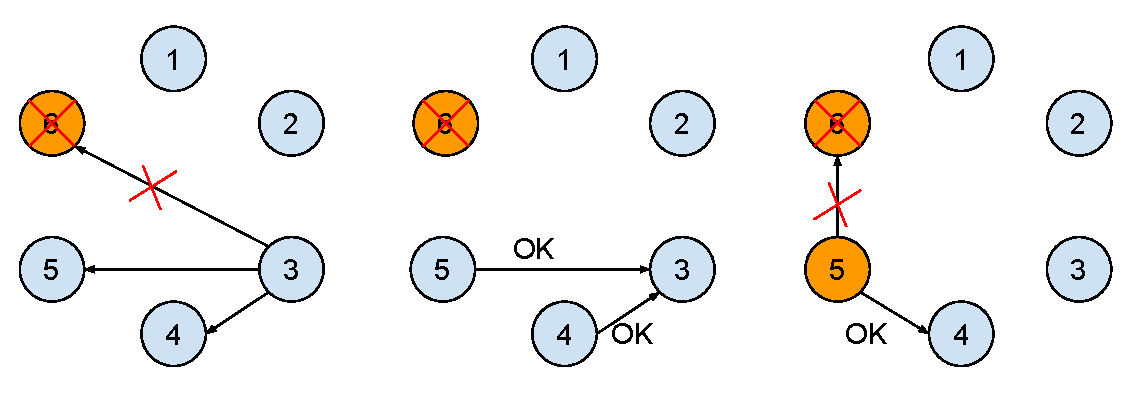
\includegraphics[width=0.5\textwidth]{bully}
    \caption{Example of how the bully algorithm works, the leader changes from 6 to 5}
    \label{fig:bully}
\end{figure}

\subsection{Ring algorithm election}
Every node needs to know only about his successor. When any process figures out that there is no leader anymore, it generates an election message. The message flows through the ring network and every node adds its ID in it. If a node finds its ID in the message it means that that node started the election, so it will be the new leader and a new message will be sent to announce the new coordinator. In the Fig \ref{fig:ring} the node 5 realize that the coordinator is down. It start a new election and at the end it gets the leader role. Then it sends an ok message which tells to the other nodes who is the new coordinator.
\begin{figure}[h!]
  \centering
    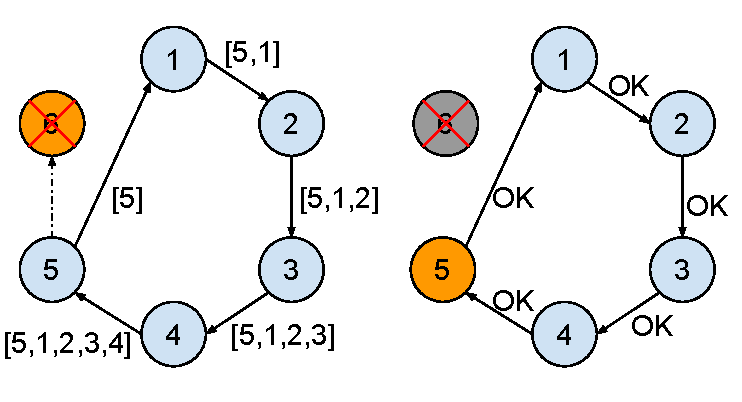
\includegraphics[width=0.5\textwidth]{ring}
    \caption{Example of how the ring algorithm election works, the leader changes from node 6 to node 5, the election is started from the node 5}
    \label{fig:ring}
\end{figure}

A good knowledge of the problems that the scale of nodes could cause is also required, that could be related to security or data consistency. Even if the solution doesn't include the security and data consistency, it should be taken into consideration a good policy of adding and removing a node such as the way of setting the successor and predecessor for every join-leave.

\section{Design}
\label{chap:design}
Since the precode was taken from the assignment 1, where a ring network was implemented, for simplicity we decided to keep this network topology also for the assignment 2. The ring algorithm election was chosen as a leader selection method; that because in our previously network topology each nodes knows about its successor, which is also the way that the ring algorithm election works. To implement the Bully algorithm we would have added further information for each node, such as a pointer to all the nodes with an higher ID than the current one.
\newline
In our implementation each node has the characteristic showed in Fig \ref{fig:node} so it knows only about the previous node, the next one and who is the leader.
\newline
The predecessor was implemented to allow an ordered join in the network.
\begin{figure}[h!]
  \centering
    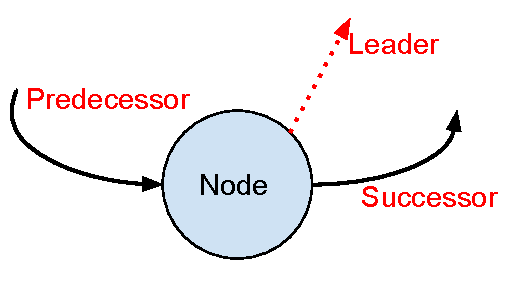
\includegraphics[width=0.5\textwidth]{node}
    \caption{Design and information stored in a single node}
    \label{fig:node}
\end{figure}

The network was designed, as the Fig \ref{fig:design} shows, to implement the leader election in a ring network topology and it includes also a join and a graceful shut-down of the node. The detection of crashes has not been implemented in this version because not required. In the Fig \ref{fig:design} the leader is the \textit{N\_L} node and when the leader leaves the network a new election must be raised. Furthermore, an external node \textit{N+1} can join the network in the ordered position according to its ID.

\begin{figure}[h!]
  \centering
    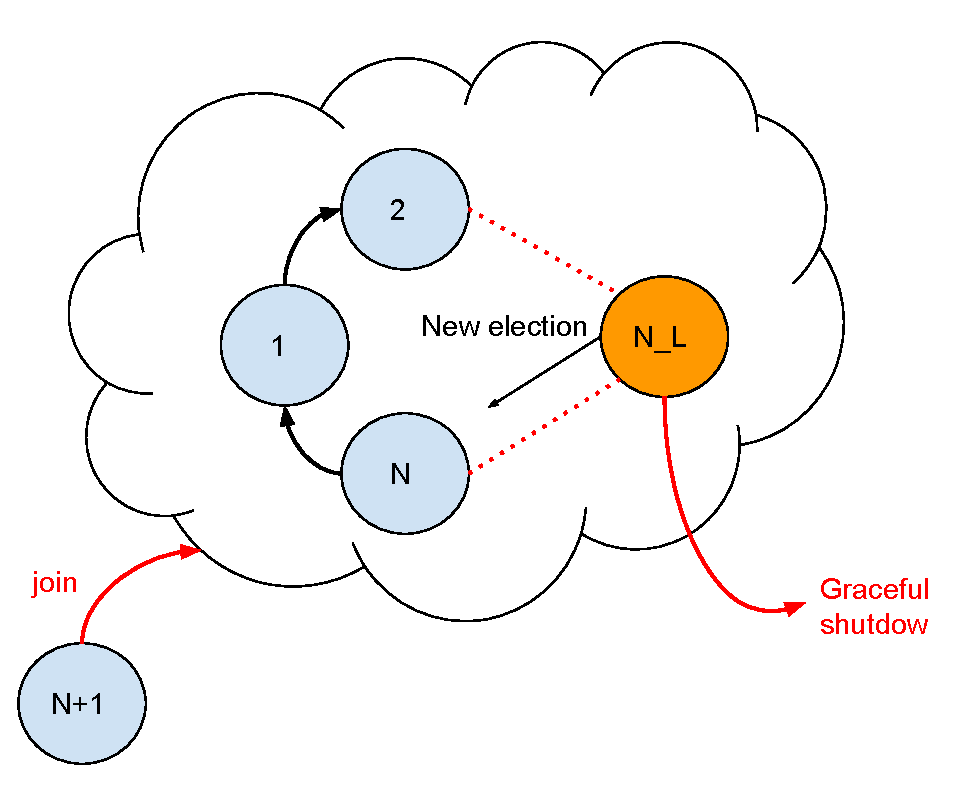
\includegraphics[width=0.5\textwidth]{design}
    \caption{Design of the implemented network}
    \label{fig:design}
\end{figure}


\section{Implementation}
As already explained in Chap \ref{chap:design}, a ring network using a ring algorithm election with join and leaving features was implemented.

The python code is made by two main classes, one in which the core of the node is stored and another which contain the \textit{HTML} parser to manage the communication between nodes. The core of the node allows to manage the following messages:
\begin{itemize}
\item[--] Join
\item[--] JoinAccepted
\item[--] NewPredecessor
\item[--] Election
\item[--] ElectionResult
\item[--] GetNeighbors
\item[--] GetLeader
\item[--] NewSuccessor 
\item[--] ShutDown
\end{itemize}

%TODO: talk about why the ring algorithm was chosen (because from the previous version of the implemented network each node has information about his successor -- which is required for the ring algorithm)

\subsection{Languages and Code}

Our solution was implemented in a mix of Python and Bash script, Python for the
actual node implementation, and a Bash script to communicate through the network created, adding and removing nodes.

We started with skeleton code by our first assignment for what concerns the node and the script code. 
The code was rearranged by removing the front-end node and by adding some properties to the nodes such as the predecessor node and information about the leader, which at the beginning, is the first node joining the network.

The code were tested before on local machine, using bash scripts and the given visual test code from Einar Holsbø Jakobsen and Magnus Stenhaug and then on the uvrocks cluster.

\subsection{Leader election}
The leader election is implemented by using the \textbf{ring algorithm election} (see Fig \ref{fig:ring}). Every node knows about which one is the leader and a new election is raised only if the current leader is gracefully shut down (chap \ref{chap:graceful}). A new election is invoked from the next-node of the previous coordinator. The election will go through all the network and each node will add its ID in a pile. When a node find its ID in the pile it will be the new leader and it will send an \textit{OK} message to all the other nodes, containing the information about who is the new leader. The Fig \ref{fig:graceful} shows the raising of a new election caused by the shutting down of the current leader $N_i$ ; is its successor, $N_{i+1}$ , which takes care to start a new election.
\newline
Since the network doesn't detect any crashes, but allows a graceful shut-down of the nodes, the problem that two nodes realise that the coordinator is missing is not taken into consideration.
\newline
The following pseudocode is called when an \textit{Election} message type is raised and represent the core implementation of the election algorithm.
\begin{lstlisting}
if no successor
    # Single node. You are already the leader
    return OK
if ID in message
    # You win. Create announce message
    announce = ElectionResult(node.next - OK)
    return OK -- with announce
else
    # add your name and forward.
    fwd = Election(add ID - node.next)
    return OK -- with fwd
\end{lstlisting}


\subsection{Join}
To implement the scaling of nodes, a \textit{join} function is fundamental together with the \textit{leave\_network} one. A node can join in every part of the network. Each node has a personal ID obtained by \textbf{hashing its IP address}. To guarantee an ordered join in the network, when a node $N_j$ asks to join to a node $N_i$ , it checks that its ID is in between the ID of $N_i$ and the ID of $N_{i+1}$ .
\newline
It is clear then, that a node $N_j$ is insert in the \textit{i} position only if the following formula is respected:
\[
N_{i} < N_j < N_{i+1}
\]
where $N_i$ is the ID number of the node which got the join request, $N_{i+1}$ the ID of its successor and $N_{j}$ the ID of the node who wants to join the network. Once that the right place is found, the properties of the new network are setted as the following:
\begin{itemize}
\item[] $\begin{aligned}
    successor(N_j) \leftarrow successor(N_i)
\end{aligned}$
\item[] $\begin{aligned}
    predecessor(N_j) \leftarrow N_i
\end{aligned}$
\item[] $\begin{aligned}
    leader(N_j) \leftarrow leader(N_i)
\end{aligned}$
\item[] $\begin{aligned}
    successor(N_i) \leftarrow N_j
\end{aligned}$
\item[] $\begin{aligned}
    predecessor(N_{i+1}) \leftarrow N_i
\end{aligned}$
\end{itemize}
A graphic implementation of the join is represented in the Fig \ref{fig:join}.
\begin{figure}[h!]
  \centering
    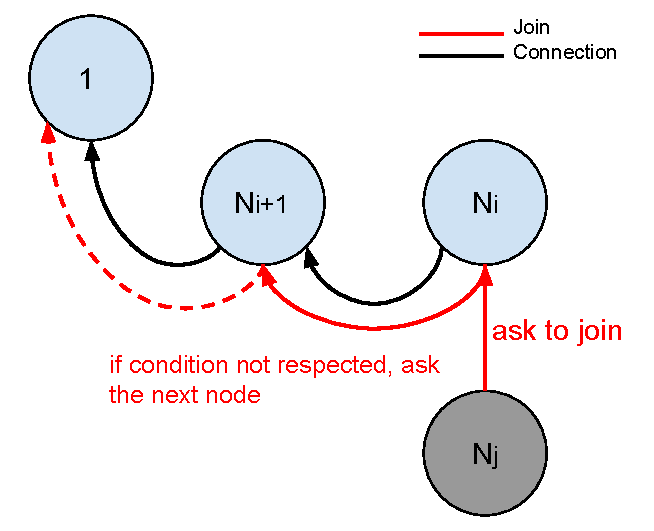
\includegraphics[width=0.5\textwidth]{join}
    \caption{Implementation of the join when a node $N_j$ ask a to a node $N_i$ to join.}
    \label{fig:join}
\end{figure}

\subsection{Graceful shut-down}
\label{chap:graceful}
The other part involved for guarantee the scalability is the \textit{node leaving} function. As said before, we don't provide fault tolerance and only a graceful shut-down of the nodes is implemented. When a simple node is shut-down, before leaving the network, it gives the information about its predecessor and successor to its neighbours. If is the coordinator that leaves the network (like in Fig \ref{fig:graceful}) then the successor of the leaving node raise an election message.
\newline
When a node $N_i$ leaves the network the following equations are implemented:
\begin{itemize}
\item[] $\begin{aligned}
    successor(N_{i-1}) \leftarrow N_{i+1}
\end{aligned}$
\item[] $\begin{aligned}
    predecessor(N_{i+1}) \leftarrow N_{i-1}
\end{aligned}$
\end{itemize}

\begin{figure}[h!]
  \centering
    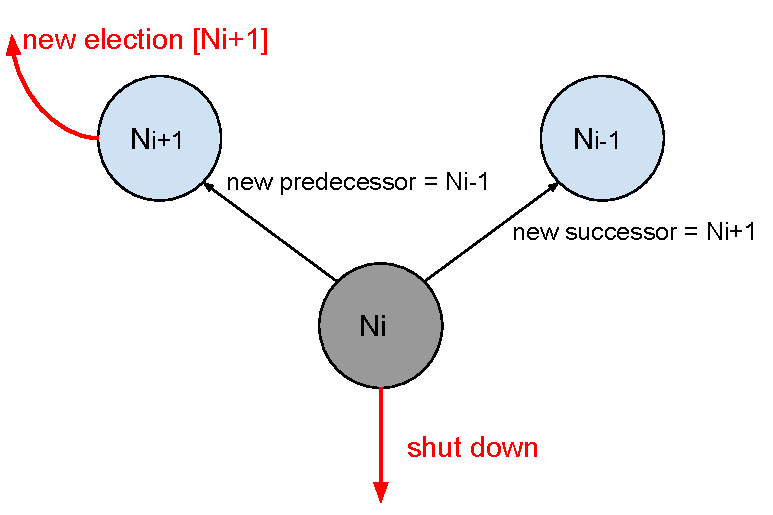
\includegraphics[width=0.5\textwidth]{graceful}
    \caption{Example of graceful shut-down on the node $N_i$, which is also the leader.}
    \label{fig:graceful}
\end{figure}

\subsection{Node}
Every node, as showed already in Fig \ref{fig:node}, keep informations about its successor, predecessor and the network leader. In each node are defined all the type of messages that it can receive or send and once they are active they are doing nothing besides waiting that some action such as a join or a leave is raised.
\newline
If a join request is raised on the node, it sends to the new node the pointer to its successor, in that way the joining node can use it as its successor in case of accept and as a next node to call in case of join refused.
If a graceful shut-down is called on the current node, it checks whether itself is the coordinator or not; if yes then raise a new election on the next node. Before going down it sends to its successor a pointer to its predecessor and to its predecessor a pointer to its successor.
\newline
When a new election is raised on the current node, it checks if its ID is in the list received (which is empty when the election begins), if yes then the current node is the new coordinator if not it puts its ID in the list and forward the election message. When the election is completed the pointer to the new leader is setted.

\subsection{Environment}
Our code was written to run on the Rocks Cluster distribution\cite{rocks}, and
makes some assumptions about that environment. We rely on the cluster's shared
filesystem for distributing program code to servers. And we rely on easy SSH
access between machines in the cluster to start and shutdown nodes.

\section{Discussion}
The leader election with the Bully algorithm is faster than the ring one because the message sent concern only the nodes with an higher ID and not all the network. However the join and leave operation with the Bully are more expensive.
Even though the Bully algorithm may be faster for what concern the leader election, an implementation with the ring algorithm election was chosen to avoid any changes to the network topology already built. The implementation was more intuitive and the information which each node has to manage are less expensive when there is a join or a leave. Indeed with the Bully algorithm implementation each node need to know informations about every node with an higher ID, so for each join is necessary to involve the whole network, it doesn't matter if the position choose is already the right one; in our implementation instead, the only nodes involved are the neighbours of the node which get the join request and eventually the next nodes if the position requested is not immediately the right one. Is good to take this into consideration because if the network has a very frequent and high variation of number of nodes then is preferred to have a faster implementation of the join and leave than a faster leader election.
\newline
If we consider \textbf{fault tolerance} is good to analyse how to act in case of crashes. A simple solution could be implementing for each node a \textit{next\_next node} pointer, which means that if a node $N_i$ can't reach the node $N_{i+1}$ it jumps directly to the $N_{i+2}$ and the $N_{i+1}$ is considered out of the network. The side effect is if two consecutive nodes crash at the same time. Another thing to consider could be if two nodes crash at the same time and one of them was the coordinator. With the \textit{next\_next node} pointer it could be that two nodes realise at the same time that the leader is missing so they both start a new election.
\newline
The \textit{join} and \textit{leave} could cause some problems to the network if two or more nodes are added or removed in a really short period of time. The same problem could be raised if during an election there are nodes joining or leaving the network. This could be solved by implementing a \textbf{state machine} in the network. In that way if the network is in the \textit{insert} status won't be possible to insert, remove or start a new election for anyone inside the network until the status is not back in \textit{ready} (Fig \ref{fig:state_machine}). However, we decided that the effort to solve this little issue was not worthy for the purpose of this assignment.  
\begin{figure}[h!]
  \centering
    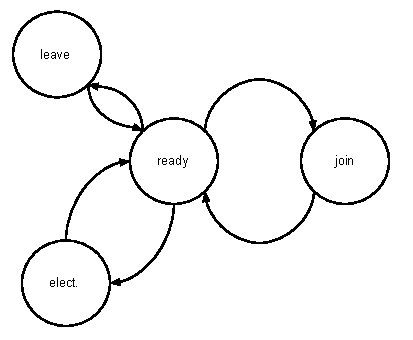
\includegraphics[width=0.5\textwidth]{state_machine}
    \caption{Possible implementation of the State Machine in the network}
    \label{fig:state_machine}
\end{figure}


\section{Evaluation}
%TODO: TEST TIME OF ELECTION WITH DIFFERENT NUMBER OF NODES (SCALING). Test also the join time(optional)

For the evaluation the scaling on the nodes executing the election algorithm has been considered.
In the Fig \ref{tab:scaling} there are the data collected considering the number of node used in the network and the respectively time to perform the election algorithm. 
\begin{figure}[h!]
\centering
% \renewcommand{\figurename}{Fig.}
\caption{Time to perform the election algorithm using \textit{n} number of nodes}
\begin{tabular}[H]{ | l | l | }
\hline
	Nodes & Time(s) \\ \hline
	2 & 0,003 \\ \hline
	5 & 0,006 \\ \hline
	10 & 0,014 \\ \hline
	15 & 0,021 \\ \hline
	19 & 0,029 \\ \hline
\end{tabular}
\label{tab:scaling}
\end{figure}

In the Fig \ref{fig:scaling} instead the graphic of this scaling test is characterized.


\begin{figure}[h!]
  \centering
    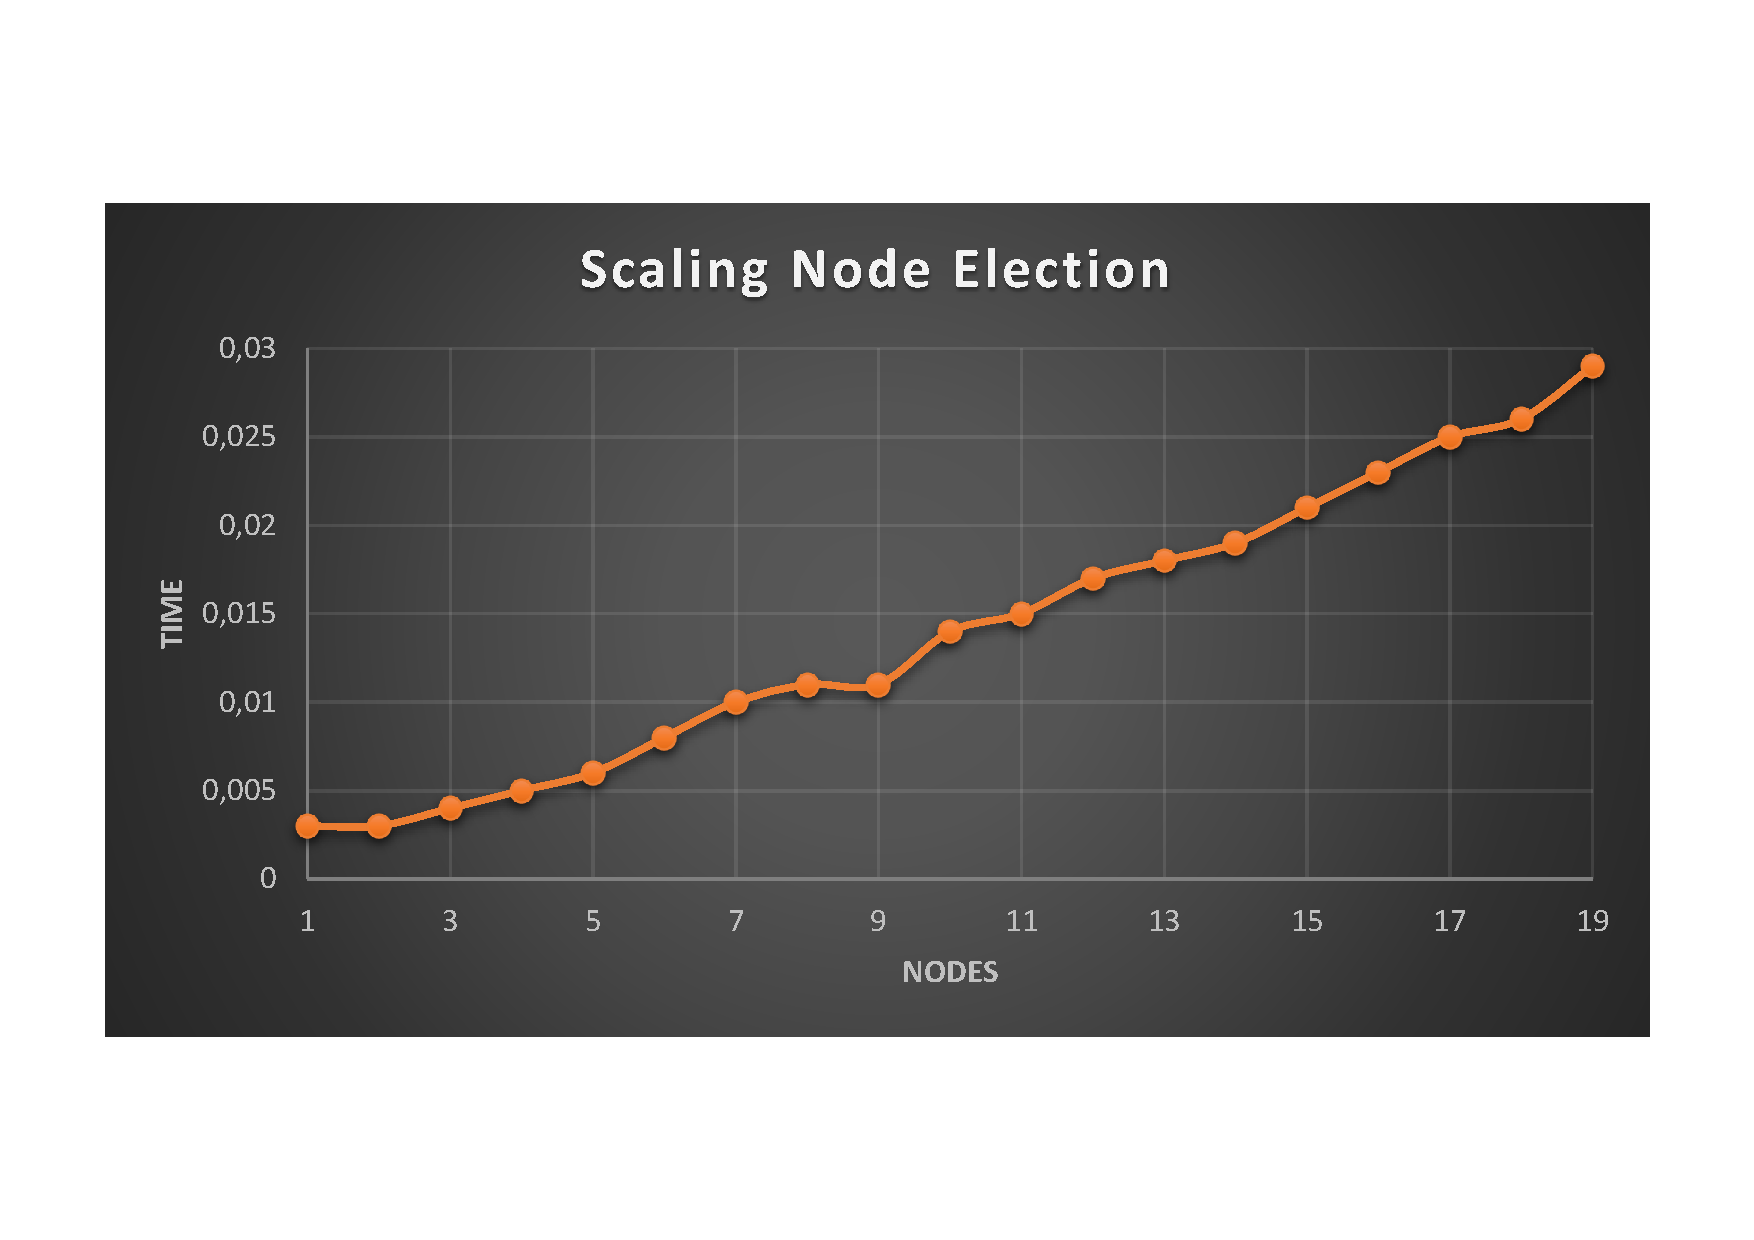
\includegraphics[width=0.5\textwidth]{scaling}
    \caption{The election algorithm time (y axis) with the relative number of node active in the network (x axis)}
    \label{fig:scaling}
\end{figure}

\section{Conclusion}

Our DHT solution, with a simple ring structure, was able to store and retrieve
data correctly, in time that increased linearly with the number of nodes
($O(n)$).


\bibliographystyle{plain}
\bibliography{report}


\end{document}
